\label{sec:sheriffframework}


%%%%%%%%%%%%%%%%%%%%%%%%%%%%%%%%%%%%%%%%%%%%%%%%%%%%%%%
% How to replace threads with processes ?
%  1. Replacing pthread_create() with fork
%  2. How to achieve the same semantics with multithreading? 
%     a. Thread Creation and Exits
%     b. Synchronizations?
%     c. Custom Memory Allocator. how to share memory across different threads
%     d. Twinning and diffing mechanism
%
%%%%%%%%%%%%%%%%%%%%%%%%%%%%%%%%%%%%%%%%%%%%%%%%%%%%%%%

\sheriff{} extends the processes-as-threads idea, first introduced in Grace~\cite{grace}, to be a drop-in replacement  of the standard \pthreads{} library. It interposes those thread-spawning calls and replaces them with \texttt{clone} system calls with \texttt{CLONE\_FILES} flag, turning threads into processes. Since different processes have separate address spaces and signal handlers, different processes can isolate their executions and employ page-based ``per-thread'' memory protection. In order to achieve the shared-memory semantics of multithreaded programs, \sheriff{} replaces synchronizations with process-based synchronizations (Section~\ref{sec:sheriffsync}), runs the regions between synchronizations in the isolation mode (Section~\ref{sec:sherifftransaction}), and commits process-private changes to the shared mapping (Section~\ref{sec:sharedmemory}). 

\begin{figure*}[!h]
\centering
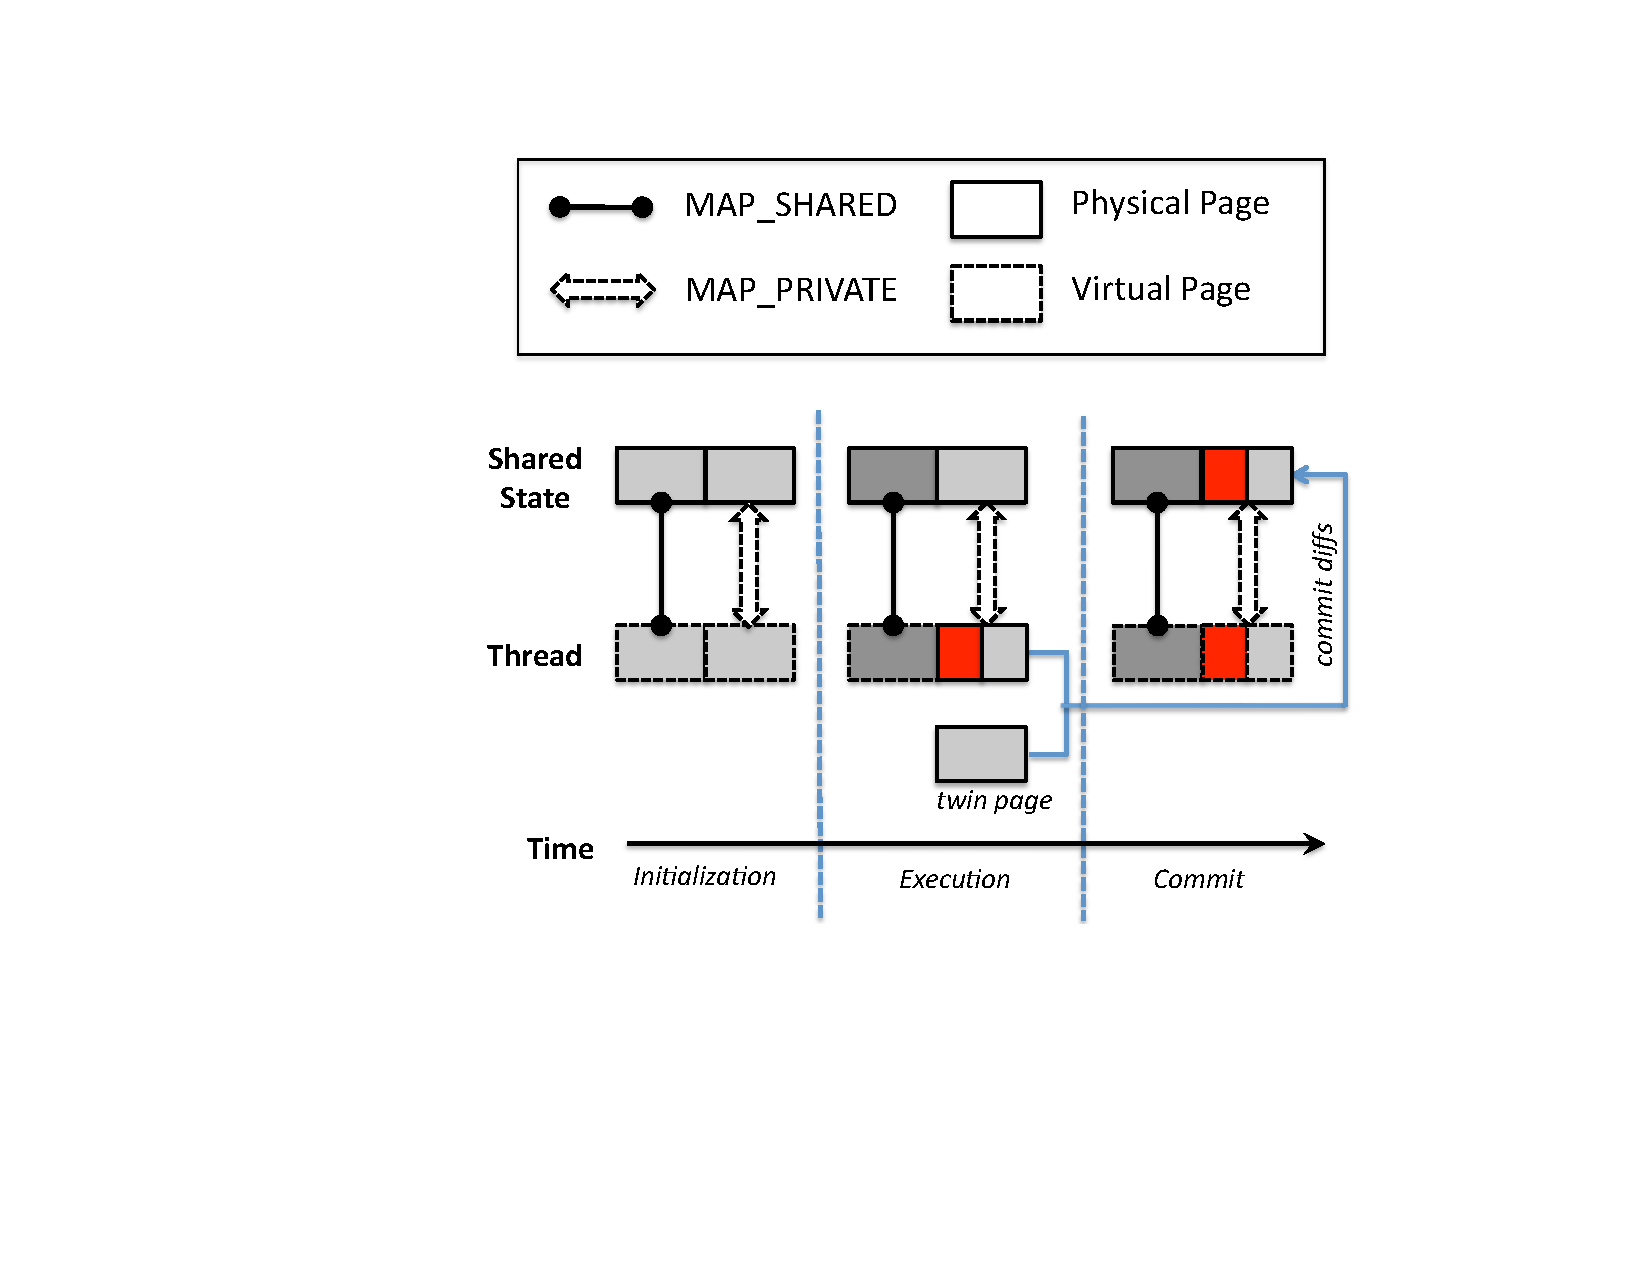
\includegraphics[height=6in]{sheriff/figure/sheriffframework.pdf}
\caption{
\Sheriff{} replaces threads with processes, thus it enables page-based ``per-thread'' memory protection and memory isolation. Upon synchronization points, local changes of different ``threads'' are committed to the shared state by comparing the difference between those working pages and their twin pages. \label{fig:overview}}
\end{figure*}

\section{Thread Creation and Exit}
\label{sec:threadcreat}

For thread creations, \sheriff{} interposes \texttt{pthread\_create()} functions and replaces them with \texttt{clone} system calls. 
By taking advantage of a feature of Linux that allows
selective sharing of memory and file descriptors, \sheriff{}
sets the \texttt{CLONE\_FILES} flag when creating new processes, resulting in child processes with different address spaces but the same shared file descriptor table. However, this attribute may not be applicable to other systems, e.g., Solaris. That would require shims on I/O operations to allow processes to share open file descriptors by sending
them over UNIX domain sockets~\cite[Section 17.4]{unixprogramming}.

For those children threads, \sheriff{} specifically invokes the \texttt{exit} function in order to exit those processes. For \texttt{pthread\_join}, joiners call \texttt{waitpid} to wait for a corresponding process to complete.  

\section{Synchronizations}
\label{sec:sheriffsync}

\sheriff{} supports the full range of synchronizations, including mutexes, conditional variables, barriers, and signals. 

By definition, synchronization is used to coordinate activities and data accesses among different threads. For example, a program calls \texttt{mutex\_lock()} before accessing the shared data. Leveraging on the processes-as-threads mechanism, \sheriff{} actually runs the regions between synchronizations in an isolated mode, which actually divides a program execution into different ``transactions.'' In the same transaction, all reads/writes happen only on private pages after the first write operation on those pages. Reads still perform on the shared mapping directly if a page is not written by the current thread.

At synchronization points, \sheriff{} commits those private changes of each thread to the shared mapping in order to achieve the shared memory semantics of multithreaded programs. Detailed implementation about the execution inside a transaction is discussed in Section~\ref{sec:sherifftransaction}. 

It is noted that the transaction concept here is different from that of transactional memory~\cite{transaction}. \sheriff{} does not support rollback and favors more on a longer transaction to better amortize the overhead. 

\sheriff{} turns threads into processes and runs an application in an isolated mode when there is no synchronization. But this isolation mechanism should not work for those synchronization variables. For example, in the mutex\_lock(), if a process only updates its private page holding this lock variable, then this update is not seen by other processes, which can cause multiple processes to enter into the same critical section concurrently. In order to coordinate different threads, \sheriff{} invokes process-based synchronizations on those synchronization variables that are shared across different processes, shown in Figure~\ref{fig:synccode}. Whenever there is a synchronization, \sheriff{} ends the current transaction, gets its process-shared variable, and synchronizes on this variable by using a process-based synchronization. To quickly locate its process-shared variable for a synchronization variable, \sheriff{} simply stores the pointer of it into the first word of this synchronization variable. 
 
\begin{figure}[!t]
\small
\begin{lstlisting}[style=tt]
void sync(var) {
  endTransaction();
  realVar = getRealVariable(var);
  sync_process_based(realVar);	
  beginTransaction();
}
\end{lstlisting}
\caption{Pseudo-code for a synchronization.\label{fig:synccode}}
\end{figure}

\section{Shared Memory Semantics}
\label{sec:sharedmemory}

In order to create the shared memory illusion for the process-as-threads framework, \sheriff{} employs the memory-mapped files to share the heap and globals across different processes, but not the stack. Different threads are using their own stacks and the stack is not used as a cross-thread communication in general.

\sheriff{} creates two different mappings for both the heap and the globals. One is a shared mapping, which is used to hold the shared state. Another is a private, copy-on-write(COW) mapping (per-process) that each process works on directly. User applications can only access  private mappings. 

Private mappings are linked to shared mappings through the same memory mapped file. In the isolated mode, reads initially go to the shared mapping until the first write on a page. After the first write operation, both reads and writes happen on the private mappings only. In order to achieve the shared memory illusion, \sheriff{} commits the current thread's local changes to the shared mapping at synchronization points using the twinning-and-diffing mechanism described in Section~\ref{sec:twinning-and-diffing}. More details of this are discussed in Section~\ref{sec:sherifftransaction}.

In the initialization phase, \sheriff{} checks its \texttt{/proc/pid/maps} file to find the range of its globals and creates a shared mapping for the globals. For the heap, \sheriff{} uses a customized memory allocator, which is discussed in Section~\ref{sec:customheap}. 

\subsection{Twinning-and-Diffing mechanism}
\label{sec:twinning-and-diffing}
In order to find out those local changes made by each thread, \sheriff{] borrows the twin page mechanism, which is introduced in TreadMarks and Munin~\cite{dsm:treadmarks, dsm:munin} for tracking modifications on a page in the distributed share memory system.

The basic idea is to create an additional ``twin'' page before the actual modification, by handling those memory protection faults. It is essential to ensure that the ``twin'' page is identical to its ``working'' page. To achieve this target, \sheriff{} issues a write operation to the original page, which specifically invokes a copy-on-write operation to create a ``working'' page. Then \sheriff{} creates a ``twin'' page by copying this ``working'' page. At synchronization points, \sheriff{} compares the ``twin'' page and its ``working'' page, using a byte-by-byte comparison, in order to find out those changes made by a thread: the difference of two pages simply implies the local changes made by the current thread. 

\subsection{Custom Memory Allocation}
\label{sec:customheap}

For the program heap, \sheriff{} replaces the default heap allocator with a BiBOP-style memory allocator, built on HeapLayers~\cite{heaplayers}. \sheriff{} pre-allocates a fixed chunk of memory from its underlying operating system using \texttt{mmap} system calls and satisfies memory allocations from this block by redirecting all memory allocations and deallocations. In the heap, all heap objects have the block size of {\it power of $2$}, using an object header to mark its status and size information. There is no split and merge operation on heap objects. If the size of an allocation is less than {\it power of 2}, \sheriff{} allocates an object with the size of the next {\it power of 2}.

In order to minimize possible false sharing induced by the memory allocator, \sheriff{} borrows a ``per-thread-heap'' idea from Hoard~\cite{Hoard}. \sheriff{} divides the heap into a fixed number of sub-heaps (currently 16), with the shared metadata of the super heap.  A thread can only allocate memory from its own sub-heap. When an object is freed, this object is returned to the subheap owned by the current thread. Since the subheap of each thread is allocated from different pages, this custom memory allocator is unlikely to allocate two objects from different threads on the same cache line, helping reduce the false sharing effect. 

\section{Execution of a Transaction}
\label{sec:sherifftransaction}

This section walks through an example of \sheriff{}'s execution from the beginning of a transaction to its termination. 

\emph{Transaction Begin:}
At the beginning of every transaction, \sheriff{} write-protects all shared pages so that later writes to these pages can be caught by handling SEGV protection faults.  

\emph{Inside a Transaction: }
Inside each transaction, \sheriff{} runs at the
same speed as a conventional multithreaded program for program reads. However, the first write to a protected page triggers a page fault that \sheriff{} handles: in the page fault handler, \sheriff{} obtains an exact copy of this page (a ``twin'' page), records the page holding the faulted address, and then unprotects this page so that future accesses run at full speed. Since \sheriff{} only exposes the private mapping to user applications, write accesses on a private mapping actually create a ``working'' page for every page written inside a transaction. 

Although protection faults are expensive,
these costs are amortized over the entire transaction because each page only incurs at most one page fault per transaction.
 
\emph{Transaction End:}
At the end of each transaction, at thread exits and before synchronization points, \sheriff{} commits local changes of a thread to the shared mapping to achieve the shared memory semantics. \sheriff{} commits only the differences between those ``twin'' pages and their ``working'' pages, using a byte-by-byte comparison. 

After those local changes are committed, \sheriff{} reclaims memory holding ``twin'' pages and ``working'' pages. \sheriff{} issues the \texttt{madvise} call, with the \texttt{MADV\_DONTNEED} flag, to discard those ``working'' pages.  Then, the current thread can observe those changes made by other threads from now on. 
